\documentclass[smallextended]{svjour3}
\usepackage[T1]{fontenc}
\usepackage[utf8]{inputenc}
\usepackage{mathptmx}
\usepackage{amsmath,graphicx,booktabs,tabularx,url,placeins}
\usepackage[hidelinks]{hyperref}
\journalname{Computing}
\setlength{\emergencystretch}{2em}
\begin{document}
\title{Online Resource 1: Candidate-Restricted Influence Maximization: Reference Resolution, Coverage, and External Validation}
\titlerunning{Online Resource 1}
\author{Jiayue Sun \and Binbin Yong \and Junjie An \and Tianyu Bo \and Shuai Li}
\institute{Binbin Yong (corresponding author, details pending author verification) \at School of Information Science and Engineering, Lanzhou University, Lanzhou 730000, China \\
\email{yongbb14@lzu.edu.cn}}
\date{}\maketitle
\paragraph{Status.} Author-review draft. Identity, declarations and submission approval remain pending. Tables and figures are generated from frozen external outputs. The historical 42-condition study and 520-condition extension are separate evidence layers; the outcome-blind preflight is not utility evidence.

\section{Audit and reproducibility}
There are 54 configuration-defined external conditions and 468 executed arms.
The archive retains one JSON and NPZ pair per condition, source and data manifests,
world-ID hashes, candidate IDs, selected sequences, all round/candidate integer
totals and 10,000 evaluation values per arm. Reproduction checks the raw gzip
hashes before using the frozen runner. The author-review audit independently
parses topology, checks all recorded hashes and world IDs, reconstructs all
argmax/tie decisions, replays every full-candidate score matrix and all evaluation
arrays, and checks a scalar Python oracle on the first 16 worlds for each
distinct ordered selection within a graph/path/coupling. Complete replay and the
independent sampled oracle are different validation layers.

Frozen source files are unchanged. The original runner's entry checks did not
enforce actual raw hashes against the data manifest; the retrospective comparison
and new guarded wrapper address that enforcement gap without rewriting history.
ca-GrQc removes loops before collecting endpoints: raw vertex 12295 appears only
in a loop, explaining 5,241 rather than 5,242 vertices. The original prose was
ambiguous about endpoint collection order, while the processed size/hash were
already frozen before outcomes. Results refer to that processed graph.

Direction is part of the simulation definition. CollegeMsg goes from sender to
receiver; wiki-Vote from voter to votee; ca-GrQc uses reciprocal arcs. The first
two are directed observed relations, not measured causal diffusion. PageRank uses
standard incoming importance, while the objective follows outgoing propagation.
Direction diagnostics are post-hoc and do not isolate a causal mechanism.

\section{Statistical interpretation}
For a fixed selected pair, conditional Monte Carlo standard error is the sample
standard deviation of 10,000 paired per-world differences divided by 100.
Normal intervals are pointwise and conditional. Across-path SD describes five
computational paths, or three control paths, and includes finite evaluation noise.
The optional $t$ intervals in CSVs are post-hoc descriptive intervals, not
population-of-network inference. Random pools are averaged within each path
before cross-path analysis; their shared-world covariance is retained.

Incremental spread subtracts five seeds from total spread. Percentage loss is
minus the paired mean difference divided by full incremental spread, times 100.
The plug-in percentage does not have a guaranteed loss-bound interpretation.
The primary sign-test family is three methods within each graph at $W=1280$.
All nonzero PageRank and random-mean differences are negative, but five paths
limit the minimum two-sided exact sign-test value to .0625. Nonsignificance is
not equivalence. Table~\ref{tab:tests} reports all nine tests without exclusions.

\section{Cost and repeated measurements}
The archived preparation timer contains parsing, all rankings, hashes and graph
diagnostics. Its ranking subtimers are not added to it again. A separate
post-hoc setup study measures five repetitions of raw parsing/CSR and one
method's ranking plus pool generation. The frozen selection timer already includes
lexical candidate sorting; it is not charged again. Hybrid deployment cost adds that
median setup to frozen selection-world preparation and selection. Hybrid
verification cost adds independent-world preparation and independent evaluation.
These are assembled warm-process, cached-file estimates, not direct end-to-end
trials. Imports, JIT compilation, downloads and output writing are excluded.

Frozen repeated timing uses path 1101 and $W=320$, five randomized repetitions
per arm, yielding 130 observations. Selected sequences and per-world evaluations
were required to remain identical. The CSVs report every repetition and its
selection/evaluation time, plus medians and ranges. The maximum positive psutil
process-lifetime peak is 3.448822 GiB; it must not be confused with an unverified
PowerShell display or with preflight measurements using one tenth the evaluation
world count. Timings are machine- and implementation-specific.

\section{Complete aggregate results}
Tables~\ref{tab:s-ca_grqc}--\ref{tab:s-wiki_vote} retain every method at all external
budgets/couplings. Total spread, paired difference, between-path SD, percentage
incremental loss and ordered agreement are shown. CSVs additionally retain
candidate fractions, set agreement, Jaccard, first divergence, conditional
uncertainty, costs and every path. This avoids treating an averaged random seed
set as if it existed. There were no failed or excluded main conditions.
\begin{table}[htbp]
\caption{Prespecified primary exact two-sided sign tests at $W=1280$. Holm correction is across three methods within each fixed graph. Zero path differences are dropped from the sign test.}\label{tab:tests}
\begin{tabular}{llrrrr}
\toprule
Graph & Method & Mean $\Delta$ & Zeros & $p$ & Holm $p$ \\
\midrule
CollegeMsg & Degree 4k & 0.00000 & 5 & 1.0000 & 1.0000 \\
CollegeMsg & PageRank 4k & -0.90780 & 0 & 0.0625 & 0.1875 \\
CollegeMsg & Random mean & -8.22745 & 0 & 0.0625 & 0.1875 \\
ca-GrQc & Degree 4k & 0.00000 & 5 & 1.0000 & 1.0000 \\
ca-GrQc & PageRank 4k & -0.25082 & 0 & 0.0625 & 0.1875 \\
ca-GrQc & Random mean & -3.94366 & 0 & 0.0625 & 0.1875 \\
wiki-Vote & Degree 4k & 0.00000 & 5 & 1.0000 & 1.0000 \\
wiki-Vote & PageRank 4k & -40.69334 & 0 & 0.0625 & 0.1875 \\
wiki-Vote & Random mean & -50.90179 & 0 & 0.0625 & 0.1875 \\
\bottomrule
\end{tabular}
\end{table}

\clearpage
\begin{table}[htbp]
\caption{ca-GrQc: complete frozen aggregate matrix; PageRank uses default tolerance. E means fixed-edge coupling (three paths); other rows use five step-coupled paths. SD is across path mean differences. Random pools are averaged within each path; their agreement entry is a fraction.}\label{tab:s-ca_grqc}
\begin{tabular}{rlrrrrr}
\toprule
$W$ & Method & Total & $\Delta$ & SD & Loss (\%) & Order \\
\midrule
80 & Degree 4k & 9.636 & +0.226 & 0.190 & -5.16 & 1/5 \\
80 & Degree 5\% & 9.410 & +0.000 & 0.000 & 0.00 & 5/5 \\
80 & Full & 9.410 & +0.000 & 0.000 & 0.00 & 5/5 \\
80 & PageRank 4k & 9.646 & +0.236 & 0.274 & -5.61 & 0/5 \\
80 & PageRank 5\% & 9.522 & +0.111 & 0.125 & -2.62 & 2/5 \\
80 & Random mean & 5.961 & -3.449 & 0.303 & 78.14 & 0.00 \\
320 & Degree 4k & 9.845 & +0.038 & 0.086 & -0.83 & 4/5 \\
320 & Degree 5\% & 9.806 & +0.000 & 0.000 & 0.00 & 5/5 \\
320 & Full & 9.806 & +0.000 & 0.000 & 0.00 & 5/5 \\
320 & PageRank 4k & 9.680 & -0.126 & 0.181 & 2.53 & 0/5 \\
320 & PageRank 5\% & 9.806 & +0.000 & 0.000 & 0.00 & 5/5 \\
320 & Random mean & 5.983 & -3.824 & 0.272 & 79.50 & 0.00 \\
1280 & Degree 4k & 9.934 & +0.000 & 0.000 & 0.00 & 5/5 \\
1280 & Degree 5\% & 9.934 & +0.000 & 0.000 & 0.00 & 5/5 \\
1280 & Full & 9.934 & +0.000 & 0.000 & 0.00 & 5/5 \\
1280 & PageRank 4k & 9.683 & -0.251 & 0.076 & 5.07 & 0/5 \\
1280 & PageRank 5\% & 9.934 & +0.000 & 0.000 & 0.00 & 5/5 \\
1280 & Random mean & 5.990 & -3.944 & 0.221 & 79.90 & 0.00 \\
320E & Degree 4k & 9.934 & +0.082 & 0.079 & -1.70 & 1/3 \\
320E & Degree 5\% & 9.852 & +0.000 & 0.000 & 0.00 & 3/3 \\
320E & Full & 9.852 & +0.000 & 0.000 & 0.00 & 3/3 \\
320E & PageRank 4k & 9.689 & -0.162 & 0.086 & 3.33 & 0/3 \\
320E & PageRank 5\% & 9.904 & +0.052 & 0.090 & -1.09 & 2/3 \\
320E & Random mean & 6.108 & -3.744 & 0.137 & 77.16 & 0.00 \\
\bottomrule
\end{tabular}
\end{table}

\clearpage
\begin{table}[htbp]
\caption{CollegeMsg: complete frozen aggregate matrix; PageRank uses default tolerance. E means fixed-edge coupling (three paths); other rows use five step-coupled paths. SD is across path mean differences. Random pools are averaged within each path; their agreement entry is a fraction.}\label{tab:s-college_msg}
\begin{tabular}{rlrrrrr}
\toprule
$W$ & Method & Total & $\Delta$ & SD & Loss (\%) & Order \\
\midrule
80 & Degree 4k & 14.919 & +0.000 & 0.000 & 0.00 & 5/5 \\
80 & Degree 5\% & 14.919 & +0.000 & 0.000 & 0.00 & 5/5 \\
80 & Full & 14.919 & +0.000 & 0.000 & 0.00 & 5/5 \\
80 & History 4k & 14.597 & -0.322 & 0.229 & 3.21 & 0/5 \\
80 & History 5\% & 14.919 & +0.000 & 0.000 & 0.00 & 5/5 \\
80 & PageRank 4k & 13.991 & -0.928 & 0.295 & 9.33 & 0/5 \\
80 & PageRank 5\% & 14.461 & -0.457 & 0.297 & 4.57 & 0/5 \\
80 & Random mean & 6.804 & -8.114 & 0.146 & 81.84 & 0.00 \\
320 & Degree 4k & 15.019 & +0.000 & 0.000 & 0.00 & 5/5 \\
320 & Degree 5\% & 15.019 & +0.000 & 0.000 & 0.00 & 5/5 \\
320 & Full & 15.019 & +0.000 & 0.000 & 0.00 & 5/5 \\
320 & History 4k & 14.820 & -0.199 & 0.130 & 1.97 & 0/5 \\
320 & History 5\% & 15.019 & +0.000 & 0.000 & 0.00 & 5/5 \\
320 & PageRank 4k & 14.164 & -0.854 & 0.117 & 8.52 & 0/5 \\
320 & PageRank 5\% & 14.645 & -0.374 & 0.125 & 3.72 & 0/5 \\
320 & Random mean & 6.836 & -8.183 & 0.211 & 81.70 & 0.00 \\
1280 & Degree 4k & 15.072 & +0.000 & 0.000 & 0.00 & 5/5 \\
1280 & Degree 5\% & 15.072 & +0.000 & 0.000 & 0.00 & 5/5 \\
1280 & Full & 15.072 & +0.000 & 0.000 & 0.00 & 5/5 \\
1280 & History 4k & 14.820 & -0.252 & 0.024 & 2.50 & 0/5 \\
1280 & History 5\% & 15.072 & +0.000 & 0.000 & 0.00 & 5/5 \\
1280 & PageRank 4k & 14.164 & -0.908 & 0.041 & 9.01 & 0/5 \\
1280 & PageRank 5\% & 14.641 & -0.431 & 0.043 & 4.28 & 0/5 \\
1280 & Random mean & 6.845 & -8.227 & 0.266 & 81.69 & 0.00 \\
320E & Degree 4k & 15.062 & +0.000 & 0.000 & 0.00 & 3/3 \\
320E & Degree 5\% & 15.062 & +0.000 & 0.000 & 0.00 & 3/3 \\
320E & Full & 15.062 & +0.000 & 0.000 & 0.00 & 3/3 \\
320E & History 4k & 14.790 & -0.272 & 0.037 & 2.71 & 0/3 \\
320E & History 5\% & 15.062 & +0.000 & 0.000 & 0.00 & 3/3 \\
320E & PageRank 4k & 14.128 & -0.934 & 0.031 & 9.28 & 0/3 \\
320E & PageRank 5\% & 14.631 & -0.431 & 0.046 & 4.28 & 0/3 \\
320E & Random mean & 6.925 & -8.137 & 0.293 & 80.87 & 0.00 \\
\bottomrule
\end{tabular}
\end{table}

\clearpage
\begin{table}[htbp]
\caption{wiki-Vote: complete frozen aggregate matrix; PageRank uses default tolerance. E means fixed-edge coupling (three paths); other rows use five step-coupled paths. SD is across path mean differences. Random pools are averaged within each path; their agreement entry is a fraction.}\label{tab:s-wiki_vote}
\begin{tabular}{rlrrrrr}
\toprule
$W$ & Method & Total & $\Delta$ & SD & Loss (\%) & Order \\
\midrule
80 & Degree 4k & 60.736 & +0.000 & 0.000 & 0.00 & 5/5 \\
80 & Degree 5\% & 60.736 & +0.000 & 0.000 & 0.00 & 5/5 \\
80 & Full & 60.736 & +0.000 & 0.000 & 0.00 & 5/5 \\
80 & PageRank 4k & 20.043 & -40.693 & 0.138 & 73.01 & 0/5 \\
80 & PageRank 5\% & 46.855 & -13.882 & 0.107 & 24.91 & 0/5 \\
80 & Random mean & 9.775 & -50.961 & 1.921 & 91.43 & 0.00 \\
320 & Degree 4k & 60.736 & +0.000 & 0.000 & 0.00 & 5/5 \\
320 & Degree 5\% & 60.736 & +0.000 & 0.000 & 0.00 & 5/5 \\
320 & Full & 60.736 & +0.000 & 0.000 & 0.00 & 5/5 \\
320 & PageRank 4k & 20.014 & -40.722 & 0.112 & 73.06 & 0/5 \\
320 & PageRank 5\% & 46.986 & -13.750 & 0.250 & 24.67 & 0/5 \\
320 & Random mean & 9.831 & -50.905 & 1.897 & 91.33 & 0.00 \\
1280 & Degree 4k & 60.736 & +0.000 & 0.000 & 0.00 & 5/5 \\
1280 & Degree 5\% & 60.736 & +0.000 & 0.000 & 0.00 & 5/5 \\
1280 & Full & 60.736 & +0.000 & 0.000 & 0.00 & 5/5 \\
1280 & PageRank 4k & 20.043 & -40.693 & 0.138 & 73.01 & 0/5 \\
1280 & PageRank 5\% & 47.206 & -13.530 & 0.096 & 24.28 & 0/5 \\
1280 & Random mean & 9.834 & -50.902 & 1.892 & 91.33 & 0.00 \\
320E & Degree 4k & 60.663 & +0.000 & 0.000 & 0.00 & 3/3 \\
320E & Degree 5\% & 60.663 & +0.000 & 0.000 & 0.00 & 3/3 \\
320E & Full & 60.663 & +0.000 & 0.000 & 0.00 & 3/3 \\
320E & PageRank 4k & 20.087 & -40.576 & 0.003 & 72.90 & 0/3 \\
320E & PageRank 5\% & 47.050 & -13.613 & 0.209 & 24.46 & 0/3 \\
320E & Random mean & 9.394 & -51.269 & 1.963 & 92.11 & 0.00 \\
\bottomrule
\end{tabular}
\end{table}

\FloatBarrier
\section{Post-hoc PageRank precision control}
The frozen default tolerance is $10^{-6}$, and NetworkX stops on a successive
vector $L_1$ change below $n$ times that value. A candidate-only diagnostic at
$10^{-12}$ changed some pool members on ca-GrQc and wiki-Vote; pools agreed
between $10^{-12}$ and $10^{-14}$. Before inspecting new utility outputs, a
separate protocol froze two PageRank arms on every graph and all five original
$W=1280$ paths. Its 15 conditions and 30 arms are a numerical sensitivity control,
not independent confirmation and not additional paths in the primary tests.

Table~\ref{tab:precision} shows that tightening tolerance changes ca-GrQc's 4k
mean difference from $-0.25082$ to $+0.02608$, replacing all five selected sets.
Its original small loss is therefore not precision-robust. CollegeMsg outcomes
are unchanged. wiki-Vote's 4k loss remains large ($-41.21970$, or 73.96\% of
incremental spread), and its 5\% loss is 24.47\%. This diagnostic qualifies the
ranking interpretation without replacing any original observation or retroactively
redefining the frozen sign-test family. Tightened-solver timing is not substituted
into the default-solver cost curves.
\begin{table}[htbp]
\caption{Post-hoc precision control at $W=1280$, tolerance $10^{-12}$. Difference is versus frozen full greedy; change is versus the default PageRank implementation. Order compares with default PageRank, not full eligibility. These are the original five paths, not new independent samples.}\label{tab:precision}
\begin{tabular}{llrrrr}
\toprule
Graph & Pool & Difference & Loss (\%) & Change & Order \\
\midrule
ca-GrQc & PageRank 4k & 0.02608 & -0.54 & +0.27690 & 0/5 \\
ca-GrQc & PageRank 5\% & 0.00000 & 0.00 & +0.00000 & 5/5 \\
CollegeMsg & PageRank 4k & -0.90780 & 9.01 & +0.00000 & 5/5 \\
CollegeMsg & PageRank 5\% & -0.43094 & 4.28 & +0.00000 & 5/5 \\
wiki-Vote & PageRank 4k & -41.21970 & 73.96 & -0.52636 & 0/5 \\
wiki-Vote & PageRank 5\% & -13.63982 & 24.47 & -0.10970 & 3/5 \\
\bottomrule
\end{tabular}
\end{table}

\FloatBarrier
\section{Coupling control}
Figure~\ref{fig:coupling} shows all preselected W320 control paths for the main
ranking comparisons. Mean PageRank-4k differences under edge coupling are
$-0.16240$, $-0.93417$ and $-40.57597$ on ca-GrQc, CollegeMsg and wiki-Vote.
Degree-4k ordered agreement is 1/3, 3/3 and 3/3, respectively. This control
preserves the prominent PageRank losses while showing that coupling can change
reference reproduction. It does not estimate a general coupling-invariance law.
\begin{figure}[htbp]
\centering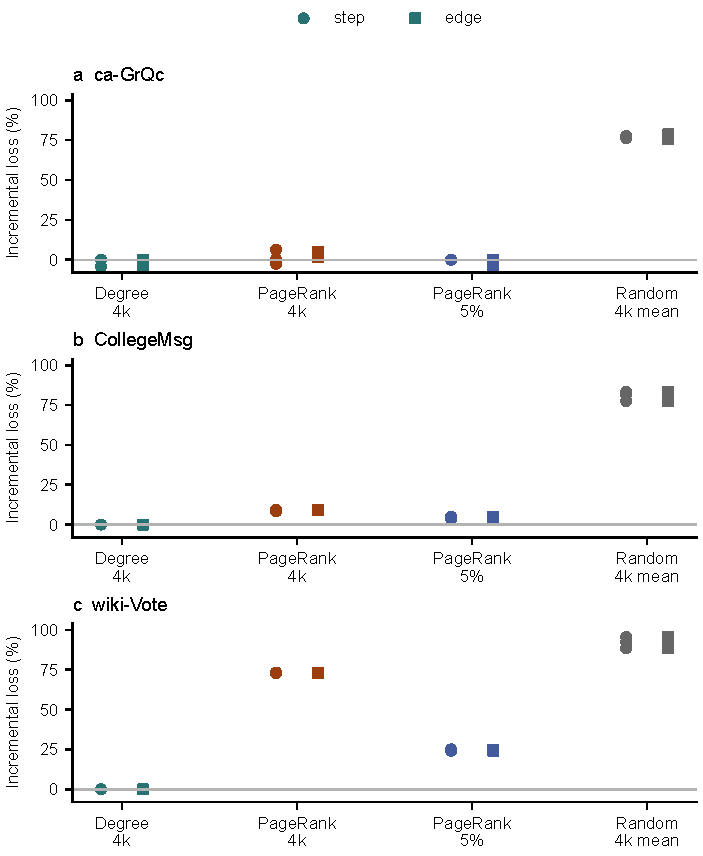
\includegraphics[width=\linewidth]{FigS1.pdf}
\caption{Coupling control at $W=320$. Each symbol is one of three preselected
computational paths, with three random-pool repetitions first averaged within
path. Circles denote step-indexed worlds and squares fixed-edge worlds. Loss is
relative to the full reference using the same coupling. No inferential intervals
are implied by these point displays}\label{fig:coupling}
\end{figure}
\FloatBarrier
\section{File map and remaining author actions}
The local review archive contains frozen configuration, source and data manifests;
all 54 result pairs; the strict audit; per-path and summary statistics; plotting
scripts and source CSVs; manuscript sources and PDFs; the novelty/evaluation
summary; a cover-letter draft; an author checklist; and environment/reproduction
instructions. A separate historical-evidence directory preserves the previous
extension and its analysis rather than merging the evidence layers.

The guarded download script obtains public sources only after checking their
expected hashes. Raw third-party archives are not redistributed. No public
archive URL is asserted. Authors must verify names, affiliations, contribution
roles, funding, conflicts, AI disclosure, permission/availability arrangements,
and approval by all authors before submission. Neither compilation success nor
this audit implies editorial acceptance or scientific approval by the authors.
\end{document}
